
\subsubsection{Use Case 4: Issue Tracking}\label{ssec:UseCase4IssueTracking}

The last use case illustrates the common Kanban usage scenario of managing issues within the field of software development. For this purpose, the \tracknshrink{DOAP} ontology will be used. \tracknshrink{DOAP} (Description of a Project) aims to describe software projects and offers a variety of properties to describe different aspects of this domain \parencite{Wilder-James}. 


\vspace*{\baselineskip}

\noindent \textsc{Outline}\\
\noindent For the subject of issue tracking, \tracknshrink{DOAP} provides a dedicated subset vocabulary (i.e., \tracknshrink{DOAP} bugs or \textit{dbug}), which will be used in the current use case.\footnote{Its specification can be found here: \url{http://ontologi.es/doap-bugs}.} The dbug vocabulary defines various properties and value ranges to describe different aspects around the topic of issue management. For example, an issue can be described by its \acrshort{dbug}\texttt{status} (e.g., new, in progress, fixed, etc.), its \acrshort{dbug}\texttt{severity} (e.g., trivial, major, critical, etc.), its initial \acrshort{dbug}\texttt{reporter}, and by other properties (see specification for references). Nevertheless, this use case aims to visualize resources (i.e., issues) by their inherent issue status value (i.e., the board’s columns), and grouped by their inherent severity value (i.e., lanes).


% \vspace*{\baselineskip}

\noindent \textsc{Board Component Resources}\\[-1.5em]

\noindent \hangindent=1.7cm \textit{Cards.}\tabto{1.7cm} The cards’ classes refer to \acrshort*{RDF} resources having their \acrshort{rdfs}\texttt{type} set to \acrshort{dbug}\texttt{issue}.\\[-1.5em]

\noindent \hangindent=1.7cm \textit{Columns.}\tabto{1.7cm} Column values are derived from a resource’s \acrshort{dbug}\texttt{status} value.\\[-1.5em]

\noindent \hangindent=1.7cm \textit{Lanes.}\tabto{1.7cm} Lanes gather resources that share the same severity value (i.e., \acrshort{dbug}\texttt{severity}).


\vspace*{\baselineskip}

\noindent \textsc{Card Component Resources}\\
\noindent Besides depicting the title and description of the issue, the \tracknshrink{DOAP} vocabulary also contains an \acrshort{dbug}\texttt{assignee} property, which shows the person assigned for an issue.


\vspace*{\baselineskip}

\noindent \textsc{Mockup}\\
\noindent \autoref{fig:RMB Use Case 4} provides a mockup of the \acrshort*{RMB} with the content requested by the board component and card component resources above. For demonstration purposes, the mockup showcases only five issues depicted by the cards of the board. The issues are separated by three columns (i.e., the \acrshort{dbug}\texttt{status} value), and two lanes (i.e., the \acrshort{dbug}\texttt{severity} value). Regarding the current use case, the prototype visualizes any set of \acrshort{RDF} issues and can update an issue’s status by dragging the corresponding card into another column.

\begin{figure}[ht]
    \libertineLF
    \centering
    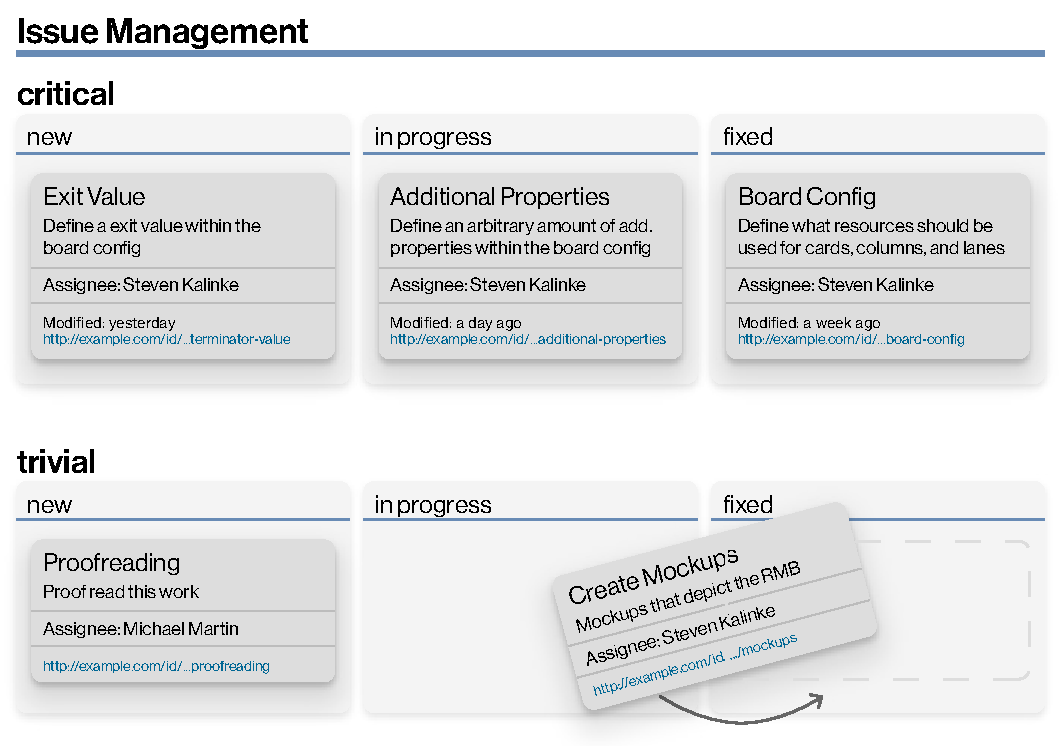
\includegraphics[width=154mm]{img/31-UseCase4.pdf}
    \caption[\tracknshrink{RMB} Mockup of Use Case 4]{\tracknshrink{RMB} Mockup of Use Case 4 depicting a mandatory title and resource identifier, and optionally a description, additional properties (i.e., assignee), and modification timestamp}.
	\label{fig:RMB Use Case 4}
\end{figure}


